\documentclass[aps,pre,preprint]{revtex4}
% \documentclass[aps,pre,twocolumn]{revtex4-1}
% \documentclass[aps,jcp,groupedaddress,twocolumn,unsortedaddress]{revtex4}

\usepackage{amsmath}
\usepackage{amssymb}
\usepackage[dvips]{graphicx}
\usepackage{color}
\usepackage{tabularx}

\makeatletter
\makeatother

\newcommand{\recheck}[1]{{\color{red} #1}}
\renewcommand{\v}[1]{\textbf{\textit{#1}}}
\renewcommand{\d}[1]{\textsf{#1}}
% \allowdisplaybreaks

\newtheorem{theorem}{Theorem}[section]
\newtheorem{lemma}[theorem]{Lemma}
\newtheorem{proposition}[theorem]{Proposition}
\newtheorem{corollary}[theorem]{Corollary}

\newenvironment{proof}[1][Proof]{\begin{trivlist}
\item[\hskip \labelsep {\bfseries #1}]}{\end{trivlist}}
\newenvironment{definition}[1][Definition]{\begin{trivlist}
\item[\hskip \labelsep {\bfseries #1}]}{\end{trivlist}}
\newenvironment{example}[1][Example]{\begin{trivlist}
\item[\hskip \labelsep {\bfseries #1}]}{\end{trivlist}}
\newenvironment{remark}[1][Remark]{\begin{trivlist}
\item[\hskip \labelsep {\bfseries #1}]}{\end{trivlist}}

\newcommand{\qed}{\nobreak \ifvmode \relax \else
      \ifdim\lastskip<1.5em \hskip-\lastskip
      \hskip1.5em plus0em minus0.5em \fi \nobreak
      \vrule height0.75em width0.5em depth0.25em\fi}


\begin{document}

\title{The Error Estimate of Force Calculation in the Inhomogeneous Molecular Systems}
\author{Han Wang}
\affiliation{LMAM and School of Mathematical
  Sciences, Peking University}
\author{Pingwen Zhang}
% \email{pzhang@pku.edu.cn}
\affiliation{LMAM and School of Mathematical
  Sciences, Peking University}

\begin{abstract}
\end{abstract}

\maketitle

\section{Theory}

\subsection{Error estimate for
  the pairwise interactions in a charged system}

In this paper, we consider the force error, bacause the applicaions
are based on the molecular dynamics simulation.  Suppose the system is
composed by $N$ charged particles located at $\v r_1, \v r_2, \cdots,
\v r_N$ with charges $q_1, q_2, \cdots, q_N$, respectively.  We study
the force error of an arbitrary charge $i$ by calculating the
difference between the exact force and calculated force exerting on
the charge $i$, which is called the \emph{error force}
\cite{wang2012} and denoted by $\Delta \v F(\v r_i)$.
% and is denoted by
% $\Delta \v F(\v r_i) = \v F(\v r_i) - \tilde{\v F}(\v r_i)$.
The maganitude of the force computation error 
% error of the force computation
is defined by the \emph{root mean square (RMS)} \emph{error}, which is
the square root of the second moment of the error force: $\mathcal
E(\v r_i) = \sqrt{\langle\vert\Delta\v F(\v r_i)\vert^2\rangle}$.  The
notation $\langle\cdot\rangle$ means ensemble average.  We also
estimate the the ensemble average of the error force (also called
\emph{mean error force}), namly $\langle\Delta\v F(\v r_i)\rangle$,
which plays an important role in the error analysis of the
inhomogeneous systems~\cite{wang2012}.

For error the pairwise interactions, we have the following theorem:
\begin{theorem}\label{thm:tmp1}
  Let a periodic molecular system be composed by $N$ charged particles
  located at $\v r_1, \v r_2, \cdots, \v r_N$ with charges $q_1, q_2,
  \cdots, q_N$, respectively.
  % Let the box vectors be $\v a_\alpha, \
  % \alpha=1,2,3$, and denote the lattice in the real space by $\v n =
  % n_1 \v a_1 + n_2 \v a_2 + n_3 \v a_3$, $n_\alpha\in\mathbb Z$.
  If the error force of an arbitary particle $i$ is
  \begin{align}\label{eqn:tmp10}
    \Delta \v F(\v r_i) =
    % \sum^\ast_{\v n}
    \sum_{j=1}^N\,q_iq_j \v K(\v r_i - \v r_j),
  \end{align}
  then the mean error force is
  \begin{align}\label{eqn:tmp11}
    \langle\Delta\v F(\v r_i)\rangle
    =q_i\, [\v K\ast\rho_q](\v r_i),
  \end{align}
  and the RMS error is
  \begin{align}\nonumber
    \mathcal E (\v r_i) 
    = &\,
    q_i^2\,[(\v K)^2\ast\rho_{q^2}] (\v r_i) + 
    q_i^2\,[\v K\ast\rho_{q}]^2 (\v r_i) \\\label{eqn:tmp12}
    &+
    q_i^2\,\int_{\mathbb R^3\times\mathbb R^3}
    \v K(\v r_i-\v r')\cdot
    \v K(\v r_i-\v r'')\,
    C_{q^2}(\v r', \v r'')\,
    \d d\v r'\d d\v r''.
  \end{align}
  Where $\ast$ denotes the convolution, and
  % The $\rho_q$, $\rho_{q^2}$ and
  % $C_{q^2}$ are defined by:
  \begin{align}\label{eqn:tmp13}
    \rho_q(\v r)
    &= 
    \bigg\langle
    \sum_{j = 1}^N
    \,q_j\,\delta(\v r - \v r_j)
    \bigg\rangle,\\\label{eqn:tmp14}
    \rho_{q^2}(\v r)
    &= 
    \bigg\langle
    \sum_{j = 1}^N
    \,q^2_j\,\delta(\v r - \v r_j)
    \bigg\rangle,\\\label{eqn:tmp15}
    C_{q^2}(\v r', \v r'')
    &=
    \bigg\langle
    \sum_{i\neq j}
    q_iq_j\delta(\v r'-\v r_i)\delta(\v r''-\v r_j)
    \bigg\rangle
    - \rho_q(\v r')\rho_q(\v r'').
  \end{align}
  Notice the definitions of $\rho_q(\v r)$, $\rho_{q^2}(\v r)$ and
  $C_{q^2}(\v r', \v r'')$ are periodically extended to
  $\mathbb{R}^3$, $\mathbb{R}^3$ and $\mathbb{R}^3\times\mathbb R^3$,
  respectively.
\end{theorem}
\begin{proof}
  By definition, the mean error force is:
  \begin{align*}
    \langle\Delta\v F(\v r_i)\rangle
    &=
    q_i\bigg\langle \sum_{j=1}^Nq_j\v K(\v r_i -\v r_j)\bigg\rangle\\
    &=
    q_i\int_{\mathbb R^3}\v K(\v r_i - \v r')
    \bigg\langle \sum_{j=1}^Nq_j\delta (\v r' -\v r_j)\bigg\rangle
    \,\d d\v r'\\
    &= 
    q_i\, [\v K\ast\rho_q](\v r_i),
  \end{align*}
  The RMS force error is calculated by:
  \begin{align*} \nonumber
    \langle\vert\Delta\v F(\v r_i)\vert^2\rangle
    =\,&
    q_i^2\bigg\langle\sum_{j,k}
    q_jq_k\v K(\v r_i - \v r_j)\cdot\v K(\v r_i - \v r_k)\bigg\rangle \\ \nonumber
    =\,&
    q_i^2\bigg\langle\sum_{j=1}^N
    q_j^2\vert\v K(\v r - \v r_j)\vert^2
    \bigg\rangle +
    q_i^2\bigg\langle\sum_{j\neq k}
    q_jq_k \v K(\v r - \v r_j)\cdot\v K(\v r - \v r_k)
    \bigg\rangle \\ \nonumber
    =\,&
    q_i^2\int_{\mathbb R^3}
    \vert\v K(\v r_i - \v r')\vert^2\rho_{q^2}(\v r')\,\d d\v r'
    \\
    & +
    q_i^2\int_{\mathbb R^3\times\mathbb R^3}
    \v K(\v r_i - \v r')\cdot\v K(\v r_i - \v r'')\,
    [\,\rho_q(\v r')\rho_q(\v r'') + C_{q_2}(\v r',\v r'')\,]
    \,\d d\v r'\d d\v r''\\
    = \,&
    q_i^2\,[(\v K)^2\ast\rho_{q^2}] (\v r_i) + 
    q_i^2\,[\v K\ast\rho_{q}]^2 (\v r_i) \\
    &+
    q_i^2\,\int_{\mathbb R^3\times\mathbb R^3}
    \v K(\v r_i-\v r')\cdot
    \v K(\v r_i-\v r'')\,
    C_{q^2}(\v r', \v r'')\,
    \d d\v r'\d d\v r''. \qquad\qed
    % \int_{\mathbb R^3\times\mathbb R^3}\v K(\v r - \v r')\cdot\v K(\v r - \v r'')\rho(\v r', \v r'')\,\d d\v r'\d d\v r''.
  \end{align*}
\end{proof}
Here are some remarks concerning Theorem~\ref{thm:tmp1}:
\begin{itemize}
\item The function $\v K(\v r)$ is called \emph{the error force
    kernel}.
  % It should be well defined for $\v r = \v 0$. For
  % the cut-off method, $\v K(\v 0) = \v 0$. For the reciprocal part 
\item The densities $\rho_q(\v r)$ and $\rho_{q^2}(\v r)$ defined in
  Eqn.~\eqref{eqn:tmp13} and \eqref{eqn:tmp14} are called \emph{the
    first order charge density distribution (CDD)} and \emph{the
    second order charge density distribution},
  respectively. $C_{q^2}(\v r, \v r')$ defined in
  Eqn.~\eqref{eqn:tmp15} is the pairwise charge correlation function.
\item Analog to the short-range error estimate~\cite{wang2012}, the
  three terms on the r.h.s. of Eqn.~\eqref{eqn:tmp12} are called the
  homogeneity error, the inhomogeneity error and the correlation
  error, respectively. The homogeneity error and the inhomogeneity
  error can be calculated at the cost of $\mathcal O(N\log N)$ by the
  fast Fourier transform (FFT) (see Ref.~\cite{wang2012} for details).
  However, the calculation of the correlation error costs $\mathcal
  O(N^2\log N)$, because it involves a twofold convolution. In this
  study, the contribution of the correlation error is neglicted.
  % In
  % section~\ref{sec:tmp3}, it is shown neglicting the 
\item A non-zero mean error force~\eqref{eqn:tmp11} was proof to be
  harmful to the simulation in the case of the short-range force
  calculation~\cite{wang2012}.  In the case of the charge system, this
  term is non-zero only when the system is NOT locally neutral. For
  most of the simulation cases, the locally neutral condition is
  satisfied, so the mean error force and the inhomogeneity error
  vanish.
  % The
  % serious artifical effect due to the inhomogeneity error of
  % short-range interaction~\cite{wang2012} does not exist in most
  % charged systems.
\end{itemize}

\subsection{Ewald summation and its error estimate}
The Ewald method divides the electrostatic interaction in to three
parts: the direct part, the reciprocal part and the correction
part. that is
\begin{equation}
E = E_{\textrm{dir}} + E_{\textrm{rec}} + E_{\textrm{corr}},
\end{equation}
where 
\begin {align}\label{eqn:tmp2}
E_{\textrm{dir}} & = \frac12 \sum^{\ast}_{\v n}
\sum_{i,j = 1}^{N} \frac{q_iq_j \textrm{erfc}(\beta \vert\v{r}_{ij} + \v{n}\vert)}
{\vert\v{r}_{ij} + \v{n}\vert} \\\label{eqn:tmp3}
E_{\textrm{rec}} & = \frac1{2\pi V} \sum_{\v m \neq 0}
\frac{\exp(-\pi^2\v m^2 / \beta^2)}{\v m^2} S(\v m) S(-\v m) \\\label{eqn:tmp4}
 E_{\textrm{corr}}& = -\frac\beta{\sqrt \pi} \sum_{i=1}^N q_i^2
\end {align}
The distance between the two particles is denoted by $\v r_{ij} = \v
r_i - \v r_j$, where $\v r_i$ and $\v r_j$ are positions of particle
$i$ and $j$, respectively.  The lattice in the real space is denoted
by $\v n = n_1 \v a_1 + n_2 \v a_2 + n_3 \v a_3$, where $\v a_\alpha,
\ \alpha=1,2,3$ are box vectors. the structure factor $S(\v m)$ is
defined by
\begin{equation}\label{sm1}
S(\v m) = \sum_{j=1}^N q_j \exp (2 \pi i \v m \cdot \v r_j),
\end{equation}
where $\v m = m_1 \v a_1^\ast + m_2 \v a_2^\ast + m_3 \v a_3^\ast$ is
the reciprocal space lattice vectors. $\v a_\alpha^\ast,\ \alpha = 1,
2, 3$ are conjugate reciprocal vectors of $\v a_\alpha$, defined by
$\v a_\alpha \cdot \v a_\beta^\ast = \delta_{\alpha\beta}$. and $V =
\v a_1 \cdot \v a_2 \times \v a_3$ is the volume of the box.

The complementary error function $\textrm{erfc}(r)$ in
Eqn.~\eqref{eqn:tmp2} decays exponentially as $r$ goes to infinity.
Therefore, it is a short-range interaction in the real space, which
can be calculated by the standard cut-off and neighbor list
method~\cite{frenkel02b} at a cost of $\mathcal O(N)$.  The reciprocal
part also decays exponentially as the maganitude of the Fourier mode
$\vert\v m\vert$ increases. Therefore, in practice, the infinit
summation in Eqn.~\eqref{eqn:tmp3} is truncated, and only a finite
summation is calculated:
% Both the direct and the reciprocal parts are calculated by cut-off in
% real and reciprocal space, respectively.
% For the reciprocal part the cut-offed energy reads
\begin{align}\label{eqn:tmp6}
  E^{\textrm{tr}}_{\textrm{rec}} & =
  % \frac1{2\pi V}
  \sum_{
    \begin{subarray}{c}
      \vert m_\alpha\vert < K_\alpha/2\\
      \v m\neq 0
    \end{subarray}}
  % \frac{\exp(-\pi^2\v m^2 / \beta^2)}{\v m^2} S(\v m) S(-\v m)   
  f(\v m)\, S(\v m) S(-\v m),
\end{align}
where, for short,
\begin{align}
  f(\v m) := \frac{\exp(-\pi^2 \v m^2 / \beta^2)}{2\pi V \v m^2},
\end{align}
and $K_\alpha$ is the number of Fourier modes used on direction
$\alpha$.  The truncated reciprocal force acting on particle $i$ is
\begin{align}\nonumber
  \v F^{\textrm{tr}}_{\textrm{rec}}(\v r_i)
  &= - 
  q_i 
  \sum_{
    \begin{subarray}{c}
      \vert m_\alpha\vert < K_\alpha/2\\
      \v m\neq 0
    \end{subarray}}
  \v g(\v m) \,
  S(-\v m)\,
  e^{2\pi i\v m\cdot\v r_i}, \\\label{eqn:tmp8}
  &= - 
  \sum_j   q_iq_j
  \sum_{
    \begin{subarray}{c}
      \vert m_\alpha\vert < K_\alpha/2\\
      \v m\neq 0
    \end{subarray}}
  \v g(\v m) \,
  e^{2\pi i\v m\cdot\v r_{ij}},
\end{align}
where
\begin{align}
  \v g(\v m) = -4 \pi \v m i f(\v m).
\end{align}


% Ref.~\cite{wang2010optimizing} pointed out that it is reasonable and
% convenient to estimate the error for the direct and reciprocal part
% seperately, namely $\Delta\v F(\v r_i) = \Delta\v F_{\textrm{dir}}(\v
% r_i) + \Delta\v F^{\textrm{tr}}_{\textrm{rec}}(\v r_i)$.  The
% $\Delta\v F_{\textrm{dir}}$ and $ \Delta\v
% F^{\textrm{tr}}_{\textrm{rec}}$ denote the direct error force and
% reciprocal error force, respectively.  The superscript ``tr'' denotes
% the reciprocal force is calculated by truncating the infinite Ewald
% summation. Other superscripts are introduced later in the paper to
% denote the error force of the fast algoritms
% that treat the Ewald summation more elaborately.

Both the direct part and reciprocal part of the Ewald summation can be
written in the form of Eqn.~\eqref{eqn:tmp11}.  The direct
error force kernel is defined by:
% The direct part is a short-range interaction in real space, so it is
% usually treated by the cut-off method, which gives a error force
% kernel of
\begin{align}
  \v K^{\textrm{cut}}_{\textrm{dir}}(\v r) =
  \left\{
    \begin{aligned}
      &\,0, &\quad & r \leq r_c;\\
      &
      \Big[
      \frac{2\beta}{\sqrt\pi} e^{-\beta^2r^2} + \frac{\textrm{erfc}(\beta r)}{r}
      \Big]\frac{\v r}{r^2}
      ,& & r > r_c,
      % \frac{\textrm{erfc}(\beta\vert\v r\vert)}{\vert\v r\vert}
    \end{aligned}
  \right.
\end{align}
where $r = \vert\v r\vert$, and $r_c$ is the cut-off radius in the
real space.
% The reciprocal error force, namely the difference between
% the the exact and truncated reciprocal force, is
% \begin{align}
%   \Delta \v F^{\textrm{tr}}_{\textrm{rec}}(\v r_i)
%   = & - 
%   \sum_j\,q_iq_j
%   \sum_{\vert m_\alpha\vert \geq K_\alpha/2}
%   \v g(\v m) \,
%   e^{2\pi i\v m\cdot\v r_{ij}}.
% \end{align}
% Therefore,
The reciprocal error force kernel is given by:
\begin{align}
  \v K^{\textrm{tr}}_{\textrm{rec}}(\v r) =
  \sum_{
      \vert m_\alpha\vert \geq K_\alpha/2}
  \v g(\v m) \,
  e^{2\pi i\v m\cdot\v r}.
\end{align}
By the Therefore \ref{thm:tmp1}, the error estimate of the
truncated Ewald summation is straightforward.


% Ref. \cite{short} pointed out that the inhomogeneity error is more
% harmful than the homogeneity error, so it is interesting to analyze
% the inhomogeneity error. Apply the Fourier transform on both sides of
% Eqn. \eqref{eqn:tmp10} and \eqref{eqn:tmp18}:
% \begin{align}  
%   \langle\Delta\v F_{\textrm{dir}}\rangle^\wedge(\v m)
%   &= q_i\,\hat{\v K}^c_{\textrm{dir}}(\v m)\cdot\hat\rho_q(\v m)\\
%   \langle\Delta\v F_{\textrm{rec}}\rangle^\wedge(\v m)
%   &= -q_i\,\hat{\v K}^c_{\textrm{rec}}(\v m)\cdot\hat\rho_q(\v m)
% \end{align}
% If the charge distribution is \emph{locally} neutral, then all modes
% of the first order density distribution vanishes, and $\langle\Delta\v
% F_{\textrm{dir}}\rangle = \langle\Delta\v F_{\textrm{rec}}\rangle = 0$.




\subsection{The smooth particle mesh Ewald method}

The naive calculation of the reciprocal Ewald summation
\eqref{eqn:tmp6} will result in a computational cost of $\mathcal
O(N^2)$. It has been shown that with a careful tuning of parameter
$\beta$ and the reciprocal space truncation $K_\alpha$, the
computational cost is reduced to $\mathcal O(N^{3/2})$
\cite{perram1988asc}, which becomes not applicable when the system
size is larger than several hundreds of charged particles. Both the
particle mesh Ewald (PME) \cite{darden1993pme} and the smooth particle
mesh Ewald (SPME) \cite{essmann1995spm} methods are designed to reduce
the computational cost to $\mathcal O(N\log N)$ in nearly the same
way.  Since the SPME method is more precise \cite{deserno1998mue1} and
more popular than the PME, we will focus our discussion on the
former. All the error estimates develop by the current paper can be
easily extended to PME method.  The principle idea of the SPME method
is first to calculate the term $e^{2\pi i\v m\cdot\v r}$ on a uniform
lattice in the real space.  Therefore, all Fourier transforms can be
accerlerated by the fast Fourier transform (FFT), that is why the
computational cost of SPME is reduced to $\mathcal O(N\log N)$. Then,
for any particle position $\v r_i$, the value of $e^{2\pi i\v m\cdot\v
  r_i}$ is interpolated by the known values on the neighboring lattice
points.  The PME method uses Lagrangian interpolation, while the SPME
uses B-spline interpolation that is more precise, and has higher order
of smoothness.

The SPME method provides two possibilities of calculating the
reciprocal force. The first one is to differentiate (with respect to
the particle position) the reciprocal term of the truncated Ewald
energy and then approximate the derived force \eqref{eqn:tmp8} by the
B-spline interplation. This way is called
\emph{ik--differentiation}. The alternative way notices the high-order
smoothness of the B-spline interpolation, and derive the force by
differentiating the B-spline approximated reciprocal Ewald energy
(also truncated). This way was proposed by the original SPME paper
\cite{essmann1995spm}, and is called the \emph{analytical
  differentiation}.  It has been shown that using the same parameters,
the ik-differentiation is more precise than the analytical
differentiation, but it requres twice more FFTs, which is a bottleneck
for the communication in parallel
implementations~\cite{wang2010optimizing}. Since the SPME method is
not the point of the present paper, we refer the readers to, for
example, Ref. \cite{essmann1995spm, deserno1998mue1,
  wang2010optimizing} for details of this method.


\subsection{Error estimate of the ik-differentiation}

From the precise calculation of the reciprocal summation to the SPME
fast algorithm, the electrostatic interaction is approximated by two
steps.  The first step is the truncation of the reciprocal summation,
i.e. Eqn. \eqref{eqn:tmp6}. The second step is the approximation of
$e^{2\pi i\v m\cdot\v r}$ by B-spline
interpolation. Ref. \cite{wang2010optimizing} has pointed out that the
error due to the first step is negligible comparing with the second
step, at least for the parameters of practical interest. Numerical
examples supporting this argument in inhomogeneous systems are also
given in Section \ref{sec:tmp3}.  Therefore, to estimate the force
error, it is enough to compare the SPME force with the
\emph{truncated} Ewald force \eqref{eqn:tmp8}. 

As mentioned above, the SPME error mainly oringinated from approximate
the term $e^{2\pi i\v m\cdot\v r}$ by the B-spline
interpolation. Denote the error introduced by this approximation by
$A(\v m, \v r)\,e^{2\pi i\v m\cdot \v r}$, we are fortunate to have
the analytical expression of $A(\v m, \v r)$:
\begin{align}\label{eqn:tmp18}
  A(\v m, \v r)
  =
  \sum_{\alpha=1}^3\sum_{l\neq 0}
  \frac
  {\big(\dfrac{2\pi m_\alpha}{K_\alpha} + 2\pi l\big)^{-n}}
  {\sum\limits_{l=-\infty}^{+\infty}
    \big(\dfrac{2\pi m_\alpha}{K_\alpha} + 2\pi l\big)^{-n}}
  \bigg(
  e^{2\pi i l K_\alpha\v a^\ast_\alpha\cdot \v r} - 1
  \bigg).
\end{align}
The error force of the ik-differentiation is therfore
\begin{align}\nonumber
  \Delta\v F_{\textrm{rec}}^{\textrm{ik}}(\v r_i)
  =\;&
  q_i
  \sum_{
    \begin{subarray}{c}
      \vert m_{\alpha}\vert < K_\alpha/2\\
      \v m\neq 0
    \end{subarray}}
  \v g(\v m)\,
  A(\v m, \v r_i)\,
  e^{2\pi i\v m\cdot \v r_i}
  \sum_{j\neq i}q_j\,e^{-2\pi i\v m\cdot\v r_j} \\\nonumber
  & +\,
  q_i
  \sum_{
    \begin{subarray}{c}
      \vert m_{\alpha}\vert < K_\alpha/2\\
      \v m\neq 0
    \end{subarray}}
  \v g(\v m)\,
  e^{2\pi i\v m\cdot \v r_i}
  \sum_{j\neq i}q_j\,A(\v m, -\v r_j)\,e^{-2\pi i\v m\cdot\v r_j}\\\label{eqn:tmp19}
  & +\,
  q_i
  \sum_{
    \begin{subarray}{c}
      \vert m_{\alpha}\vert < K_\alpha/2\\
      \v m\neq 0
    \end{subarray}}
  \v g(\v m)\,
  \big[
  A(\v m, \v r_i) +
  A(\v m, -\v r_i)
  \big].
\end{align}
The last ``self-interacting term'' is zero, because of the
symmetricity of $\v g(\v m)$ and $A(\v m, \v r)$.  Unfortunately, the
error force of ik-differentiation~\eqref{eqn:tmp19} cannot be written
in the form of~\eqref{eqn:tmp11}, so the error estimate derived by
Theorem~\ref{thm:tmp1} cannot be used here. However, it is still
possible to develop the error estimate for the ik-differentiation.
Here we only want to present the key idea and the formula of the error
estimate, and leave all details to the Appendix \ref{}.  We notice the
term $e^{2\pi i l K_\alpha\v a^\ast_\alpha\cdot\v r}$ with $l\neq 0$
in Eqn.~\eqref{eqn:tmp18} introduces some high-wave-number terms in
the expression of the error estimate.  If $K_\alpha$ is large enough,
then due to the thermal fluctuation of the system, the peaks and
valleys of the high-wave-number terms may canncels in the the
emsemble-averaged error estimate.
% Based on this observation, it is
% still possible to develop the error estimate for the
% ik-differentiation.
% And if the high wave number terms are neglected,
Therefore, by neglecting these terms, it is proved that the mean error
force of the ik-differentiation is
\begin{align}
  \big\langle
  \Delta\v F_{\textrm{rec}}^{\textrm{ik}}(\v r_i)
  \big\rangle
  & \approx
  - 2 q_i
  \bigg[
  \big(
  \sum_{\alpha}\sum_{l\neq 0}\v G_{\alpha,l}
  \big)
  \ast\rho_q\,
  \bigg] (\v r_i),
\end{align}
% Also neglect the high wave number terms,
and the RMS force error is 
\begin{align}\nonumber
  \big\langle
  \vert\Delta\v F_{\textrm{rec}}^{\textrm{ik}}(\v r_i)\vert^2
  \big\rangle
  \approx&\, 
  2q_i^2
  \bigg[\,
  \big(
  \sum_{\alpha} \sum_{l\neq 0}
  \vert \v G_{\alpha,l}\vert^2
  \big)
  \ast \rho_{q^2}
  \,\bigg] (\v r_i)
  +
  4q_i^2\,
  \bigg[
  \big(
  \sum_{\alpha} \sum_{l\neq 0}  
  \v G_{\alpha,l}
  \big)^2
  \ast \rho_{q^2}\,
  \bigg] (\v r_i) \\
  &\,+
  \big\langle
  \Delta\v F_{\textrm{rec}}^{\textrm{ik}}(\v r_i)
  \big\rangle^2.
\end{align}
Where
\begin{align}
  \v G_{\alpha,l}(\v r) =
  \sum_{
    \begin{subarray}{c}
      \vert m_{\alpha}\vert < K_\alpha/2\\
      \v m\neq 0
    \end{subarray}}
  \v g(\v m)\,
  \frac
  {\big(\dfrac{2\pi m_\alpha}{K_\alpha} + 2\pi l\big)^{-n}}
  {\sum\limits_{l=-\infty}^{+\infty}
    \big(\dfrac{2\pi m_\alpha}{K_\alpha} + 2\pi l\big)^{-n}}
  e^{2\pi i\v m\cdot\v r}.
\end{align}
$G_{\alpha,l}(\v r)$ does not depends on the coordinates of particles,
so it can be calculated once and stored in a table for further uses.



\subsection{Error estimate of the analytical differetiation}

The error force of the analytical differetiation is 
\begin{align}\nonumber
  \Delta\v F_{\textrm{rec}}^{\textrm{ana}}(\v r_i)
  =\;&
  q_i
  \sum_{
    \begin{subarray}{c}
      \vert m_{\alpha}\vert < K_\alpha/2\\
      \v m\neq 0
    \end{subarray}}
  -2f(\v m)\,
  \nabla_{\v r_i}
  e^{2\pi i\v m\cdot \v r_i}
  \sum_{j\neq i}q_j\,
  A(\v m, -\v r_j)
  e^{-2\pi i\v m\cdot\v r_j} \\\nonumber
  & +\,
  q_i
  \sum_{
    \begin{subarray}{c}
      \vert m_{\alpha}\vert < K_\alpha/2\\
      \v m\neq 0
    \end{subarray}}
  -2f(\v m)\,
  \nabla_{\v r_i}
  [A(\v m, \v r_i)\,
  e^{2\pi i\v m\cdot \v r_i} ]
  \sum_{j\neq i}q_j\,
  e^{-2\pi i\v m\cdot\v r_j} \\\nonumber
  & +\,
  q^2_i
  \sum_{
    \begin{subarray}{c}
      \vert m_{\alpha}\vert < K_\alpha/2\\\nonumber
      \v m\neq 0
    \end{subarray}}
  -2f(\v m)\,
  A(-\v m, \v r_i)\,e^{2\pi i\v m\cdot \v r_i} \nabla_{\v r_i}e^{2\pi i\v m\cdot\v r_i} \\
  & +\,
  q^2_i
  \sum_{
    \begin{subarray}{c}
      \vert m_{\alpha}\vert < K_\alpha/2\\
      \v m\neq 0
    \end{subarray}}
  -2f(\v m)\,
  e^{-2\pi i\v m\cdot \v r_i}
  \nabla_{\v r_i} [\,A(\v m, \v r_i) \,e^{2\pi i\v m\cdot\v r_i}\,]  \\\nonumber
  =&\,
  \Delta\v F_{\textrm{rec}}^{\textrm{ik}}(\v r_i)\\\nonumber
  & +\,
  q_i
  \sum_{
    \begin{subarray}{c}
      \vert m_{\alpha}\vert < K_\alpha/2\\
      \v m\neq 0
    \end{subarray}}
  -2f(\v m)\,
  \v B(\v m, \v r_i)\,e^{2\pi i\v m\cdot \v r_i}
  \sum_{j\neq i}q_j\,
  e^{-2\pi i\v m\cdot\v r_j} \\\label{eqn:ana.error.force}
  & +\,
  q^2_i
  \sum_{
    \begin{subarray}{c}
      \vert m_{\alpha}\vert < K_\alpha/2\\
      \v m\neq 0
    \end{subarray}}
  -2f(\v m)\,\v B(\v m, \v r_i) 
\end{align}
With $\v B(\v m, \v r)$ defined by
\begin{align}\nonumber
  \v B(\v m, \v r)
  &=
  \nabla_{\v r_i}A(\v m, \v r)\\
  &=
  \sum_{\alpha=1}^3\sum_{l\neq 0}
  \frac
  {\big(\dfrac{2\pi m_\alpha}{K_\alpha} + 2\pi l\big)^{-n}}
  {\sum\limits_{l=-\infty}^{+\infty}
    \big(\dfrac{2\pi m_\alpha}{K_\alpha} + 2\pi l\big)^{-n}}
  2\pi i l K_\alpha\v a_\alpha^\ast\,e^{2\pi i l K_\alpha\v a^\ast_\alpha\cdot \v r} 
\end{align}
The last term in Eqn.~\eqref{eqn:ana.error.force} is due to the
self-interaction~\cite{cerutti2009staggered, ballenegger2011removal,
  neelov2010interlaced}, which does not depends on the coordinates of
particles. Therefore, it can be calculated explicitly, and substracted
from the analytical force during the simulation. The computational cost of
the self-interacting term costs is very low comparing with the SPME
force calculation.

Neglecting all high frequency terms, we have the mean error force of
analytical differetiation:
\begin{align}\label{eqn:tmp31}
  \langle \Delta\v F_{\textrm{rec}}^{\textrm{ana}}(\v r_i)\rangle
  \approx
  \langle \Delta\v F_{\textrm{rec}}^{\textrm{ik}}(\v r_i)\rangle.
\end{align}
The RMS force error is 
\begin{align}\nonumber
  \big\langle
  \vert \Delta\v F_{\textrm{rec}}^{\textrm{ana}}(\v r_i)\vert^2
  \big\rangle
  \approx&\,
  q_i^2
  \bigg[\,
  \big(
  \sum_{\alpha} \sum_{l\neq 0}
  \vert \v G_{\alpha,l}\vert^2
  \big)
  \ast \rho_{q^2}
  \,\bigg] (\v r_i) \\\nonumber
  & +\,
  q_i^2
  \bigg[
  \big(
  \sum_{\alpha}\sum_{l\neq 0}
  \vert
  \v G_{\alpha,l} + 2\pi i\,l K_\alpha F_{\alpha,l} \v a_\alpha^\ast\vert^2
  \big)
  \ast \rho_{q^2}
  \bigg]
  (\v r_i) \\ \nonumber
  & +\,
  4q_i^2\,
  \bigg[
  \big(
  \sum_{\alpha} \sum_{l\neq 0}  
  \v G_{\alpha,l}
  \big)^2
  \ast \rho_{q^2}\,
  \bigg] (\v r_i) \\\nonumber
  & +\,
  \big\langle \Delta\v F_{\textrm{rec}}^{\textrm{ana}}(\v r_i)\big\rangle ^2\\
  &+\,
  q_i^4 \sum_{\alpha}\sum_{l\neq 0}
  4\pi^2l^2K_\alpha^2\vert\v a_{\alpha}^\ast\vert^2[C_{\alpha,l}^{\textrm{self}}]^2 .
\end{align}
% The last one is a constant that stems from the self-interaction, which
% do not depends on the
Where
\begin{align}
  F_{\alpha,l} (\v r)
  &=
  \sum_{
    \begin{subarray}{c}
      \vert m_{\alpha}\vert < K_\alpha/2\\
      \v m\neq 0
    \end{subarray}}
  (-2)f(\v m)\,
  \frac
  {\big(\dfrac{2\pi m_\alpha}{K_\alpha} + 2\pi l\big)^{-n}}
  {\sum\limits_{l=-\infty}^{+\infty}
    \big(\dfrac{2\pi m_\alpha}{K_\alpha} + 2\pi l\big)^{-n}}\,
  e^{2\pi i\v m\cdot \v r},\\
  C_{\alpha,l}^{\textrm{self}}
  &= 
  \sum_{
    \begin{subarray}{c}
      \vert m_{\alpha}\vert < K_\alpha/2\\
      \v m\neq 0
    \end{subarray}}
  (-2)f(\v m)\,
  \frac
  {\big(\dfrac{2\pi m_\alpha}{K_\alpha} + 2\pi l\big)^{-n}}
  {\sum\limits_{l=-\infty}^{+\infty}
    \big(\dfrac{2\pi m_\alpha}{K_\alpha} + 2\pi l\big)^{-n}}.
\end{align}
$F_{\alpha,l} (\v r)$ and $C_{\alpha,l}^{\textrm{self}}$ 
do not depends on the coordinates of particles,
so they can be tabulated in advance for the simulation.

\subsection{The error estimate of the total force}

In the previous subsections, we estimate the error of direct part and
reciprocal part seperately. Here we provide the error estimate for the
total force. The mean of the total error force is simply:
\begin{align}
  \langle\Delta\v F^{\textrm{x}}(\v r_i) \rangle
  &=
  \langle\Delta\v F_{\textrm{dir}}(\v r_i) \rangle +
  \langle\Delta\v F^{\textrm{x}}_{\textrm{rec}}(\v r_i) \rangle,
\end{align}
where \textrm{x} can be \textrm{tr}, \textrm{ik} or \textrm{ana},
standing for the truncated Ewald summation, the ik-differentiation
and the analytical differetiation, respectively. The mean square
total force is
\begin{align}\nonumber
  \langle\,\vert\Delta\v F^{\textrm{x}}(\v r_i)\vert^2\rangle
  = \,&
  \langle\,\vert
  \Delta\v F_{\textrm{dir}}(\v r_i) + \Delta\v F^{\textrm{x}}_{\textrm{rec}}(\v r_i) 
  \vert^2 \rangle \\\nonumber
  = \,&
  \langle\,\vert\Delta\v F_{\textrm{dir}}(\v r_i)\vert^2\rangle +
  \langle\,\vert\Delta\v F^{\textrm{x}}_{\textrm{rec}}(\v r_i)\vert^2\rangle +
  2\,\langle\Delta\v F_{\textrm{dir}}(\v r_i)\rangle
  \cdot \langle\Delta\v F^{\textrm{x}}_{\textrm{rec}}(\v r_i)\rangle \\\label{eqn:tmp36}
  &
  + 2\,\textrm{Corr}(\Delta\v F_{\textrm{dir}}(\v r_i),
  \Delta\v F^{\textrm{x}}_{\textrm{rec}}(\v r_i))
\end{align}
Where $ \textrm{Corr}(\Delta\v F_{\textrm{dir}}(\v r_i), \Delta\v
F^{\textrm{x}}_{\textrm{rec}}(\v r_i))$ denotes the correlation of
$\Delta\v F_{\textrm{dir}}(\v r_i)$ and $\Delta\v
F^{\textrm{x}}_{\textrm{rec}}(\v r_i)$:
\begin{align}\label{eqn:tmp37}
  \textrm{Corr}(\Delta\v F_{\textrm{dir}}(\v r_i),
  \Delta\v F^{\textrm{x}}_{\textrm{rec}}(\v r_i))
  & =
  \langle
  \Delta\v F_{\textrm{dir}}(\v r_i)\cdot
  \Delta\v F^{\textrm{x}}_{\textrm{rec}}(\v r_i)
  \rangle -
  \langle
  \Delta\v F_{\textrm{dir}}(\v r_i)
  \rangle\cdot
  \langle
  \Delta\v F^{\textrm{x}}_{\textrm{rec}}(\v r_i)
  \rangle.
\end{align}
In Eqn.~\eqref{eqn:tmp36}, the estimates of errors
$\langle\,\vert\Delta\v F_{\textrm{dir}}(\v r_i)\vert^2\rangle $,
$\langle\,\vert\Delta\v F^{\textrm{x}}_{\textrm{rec}}(\v
r_i)\vert^2\rangle $, $\langle\Delta\v F_{\textrm{dir}}(\v
r_i)\rangle$ and $\langle\Delta\v F^{\textrm{x}}_{\textrm{rec}}(\v
r_i)\rangle $ have been established. In section \ref{sec:tmp3}, it is
shown that the correlation between the direct and reciprocal error
force can be safely neglected.


\section{Numerical tests}\label{sec:tmp3}

We consider two inhomogeneous charge system to verify our error
estimate.  The first is locally neutral and globally inhomogeneous
charge system. In the second system, the positive and negative charges
are well seperated, while the number density of the charges is
uniform.

\subsection{Example 1: locally neutral}

\begin{figure}
  \centering
  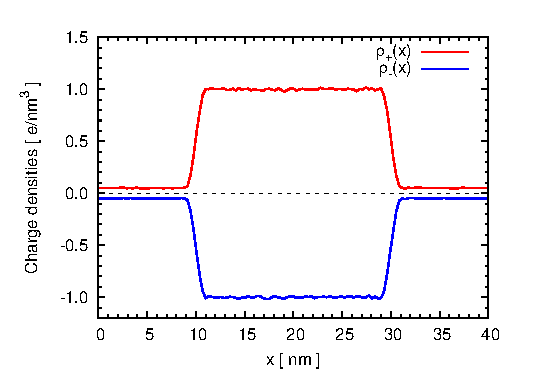
\includegraphics[width=.48\textwidth]{fig/error.one_peak.box40x20x20.b1.000.r3.00.n6.K101x051x051/fig.rho.eps}
  \caption{Charge distribution of Example 1. The red line
    denotes the positive charge distribution, while the blue line
    denotes the negative charge distribution. Since all distributions
    are uniform on $y$ and $z$ direction, they are plotted as a
    function of $x$.}
  \label{fig:tmp-rho0}
\end{figure}

In this example, 16800 charges are put into a $40\textsf{nm}\times
20\textsf{nm}\times 20\textsf{nm}$ periodic simulation box. Half of
them are carrying a unit positive charge of $+e$, and the other half
are carrying negative charge of $-e$. The position of these charges
are randomly generated subject to density distribution shown in
Fig.~\ref{fig:tmp-rho0}.  The profile of the positive and negative
charge distributions are identical, namely the minus of the negative
distribution is the same as the positive distribution. Therefore the
positive and negative charge distributions cancel each other, and the
system is locally neutral. Both the density distributions are highly
inhomogeneous, take the positive distribution for example: between 11
\textsf{nm} and 29 \textsf{nm}, the charge density is
$1.0\;\textsf{e/nm}^3$, while between 0 \textsf{nm} to 9 \textsf{nm}
and between 31 \textsf{nm} to 40 \textsf{nm}, the density is
$0.05\;\textsf{e/nm}^3$.

\begin{figure}
  \centering
  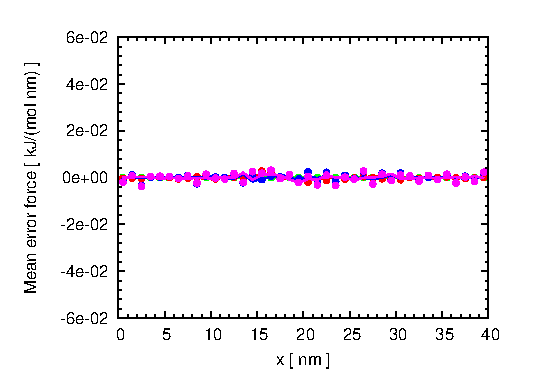
\includegraphics[]{fig/error.one_peak.box40x20x20.b1.000.r3.00.n6.K101x051x051/fig.ana.ewald.meanf.eps}
  \caption{Example 1: the actual (denoted by dots) and estimated
    (denoted by straight lines) mean error force of the direct part
    $\langle\Delta \v F_{\textrm{dir}}\rangle$ (red), reciprocal
    part of Ewald summation $\langle\Delta \v F_{\textrm{rec}}p\rangle$ (green) and the reciprocal part of the analytical
    differentiation $\langle\Delta \v
    F^{\textrm{ana}}_{\textrm{rec}}\rangle$ (blue). The total
    mean error force of analytical differentiation $\langle\Delta \v
    F^{\textrm{ana}}\rangle$ is given in pink.  Since the charge
    distribution is uniform on the $y$ and $z$ direction, the $y$ and
    $z$ dimension of the mean error force is averaged, and the errors
    are plotted on $x$ direction.  The cut-off in the real space is 3
    \textsf{nm}, the number of freedom in the reciprocal space is
    $100\times 50\times 50$, the parameter $\beta$ is $1.0\;
    \textsf{nm}^{-1}$ and the order of B-spline interpolation used for
    the analytical differentiation is 6.}
  \label{fig:meanf1}
\end{figure}

Fig.~\ref{fig:meanf1} presents the mean error force of the direct part
$\langle\Delta \v F_{\textrm{dir}}\rangle$, reciprocal part of Ewald
summation $\langle\Delta \v F_{\textrm{rec}}\rangle$ and the
reciprocal part of the analytical differentiation $\langle\Delta \v
F^{\textrm{ana}}_{\textrm{rec}}\rangle$. The total mean error force of
analytical differentiation, which is simply $\langle\Delta \v
F^{\textrm{ana}}\rangle = \langle\Delta \v F_{\textrm{dir}}\rangle +
\langle\Delta \v F^{\textrm{ana}}_{\textrm{rec}}\rangle$, is also
given.  The real and estimated mean error forces are denoted by dots
and straight lines, respectively. All estimates are consistent very
well with real errors.  Since the system is locally neutral, the first
order charge distribution $\rho_q$ is naturally zero, therefore, by
Eqn. \eqref{eqn:tmp10}, \eqref{eqn:tmp18} and \eqref{eqn:tmp31}, all
the mean error forces should varnish. Numerical resutls in
Fig. \ref{fig:meanf1} verifies with the above discussion.

\begin{figure}
  \centering
  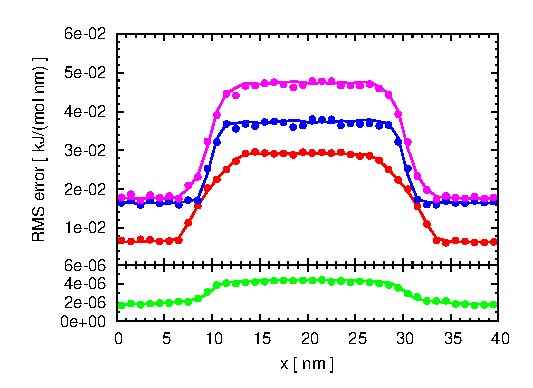
\includegraphics[]{fig/error.one_peak.box40x20x20.b1.000.r3.00.n6.K101x051x051/fig.ana.ewald.error.eps}
  \caption{Example 1: the actual (denoted by dots) and estimated
    (denoted by straight lines) RMS force error of the direct part
    $\sqrt{\langle\vert\Delta \v F_{\textrm{dir}}\vert^2\rangle}$
    (red), reciprocal part of Ewald summation
    $\sqrt{\langle\vert\Delta \v F_{\textrm{rec}}\vert^2\rangle}$
    (green) and the reciprocal part of the analytical differentiation
    $\sqrt{\langle\vert\Delta \v
      F^{\textrm{ana}}_{\textrm{rec}}\vert^2\rangle}$ (blue). The RMS
    force error of analytical differentiation
    $\sqrt{\langle\vert\Delta \v F^{\textrm{ana}}\vert^2\rangle}$ is
    given in pink.  Since the charge distribution is uniform on the
    $y$ and $z$ direction, the $y$ and $z$ dimension of the mean error
    force is averaged, and the errors are plotted on $x$ direction.
    The cut-off in the real space is 3 \textsf{nm}, the number of
    freedom in the reciprocal space is $100\times 50\times 50$, the
    parameter $\beta$ is $1.0\; \textsf{nm}^{-1}$ and the order of
    B-spline interpolation used for the analytical differentiation is
    6.}
  \label{fig:error1}
\end{figure}

Fig.~\ref{fig:error1} presents the RMS force error of the direct part
$\sqrt{\langle\vert\Delta \v F_{\textrm{dir}}\vert^2\rangle}$,
reciprocal part of Ewald summation $\sqrt{\langle\vert\Delta \v
  F_{\textrm{rec}}\vert^2\rangle}$, the reciprocal part of the
analytical differentiation $\sqrt{\langle\vert\Delta \v
  F^{\textrm{ana}}_{\textrm{rec}}\vert^2\rangle}$ and the total
analytical differentiation force $\sqrt{\langle\vert\Delta \v
  F^{\textrm{ana}}\vert^2\rangle}$.  The real and estimated mean error
forces are denoted by dots and straight lines, respectively. All the
error estimates are overlapping with the real errors, that means the
error estimates developed by the present paper are very sharp.
% Since all mean error forces varnish, the RMS force errors
% consists of only the homogeneous contribution. 
In the high charge density region, the error is comparatively larger
than the low charge density region. For the direct part, the ratio is
roughly the sqare root of the density ratio. For the reciprocal part
this ratio is lower. The reciprocal error of the analytical
differentiation is 4 orders of maganitudes large than that of the
Ewald summation, which means the Ewald summation is much more precice
than the fast algorithm based on mesh discretization.


% \begin{figure}
%   \centering
%   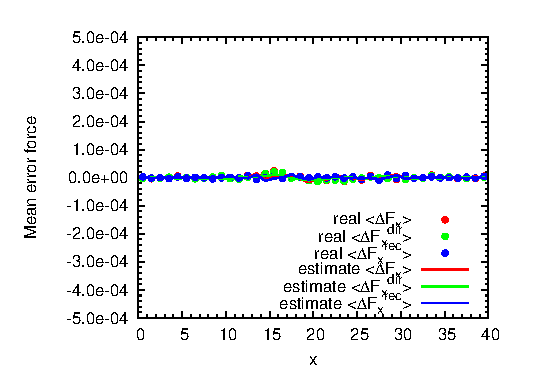
\includegraphics[width=.48\textwidth]{fig/error.one_peak.box40x20x20.b1.000.r3.00.n6.K101x051x051/fig.ik.meanf.eps}
%   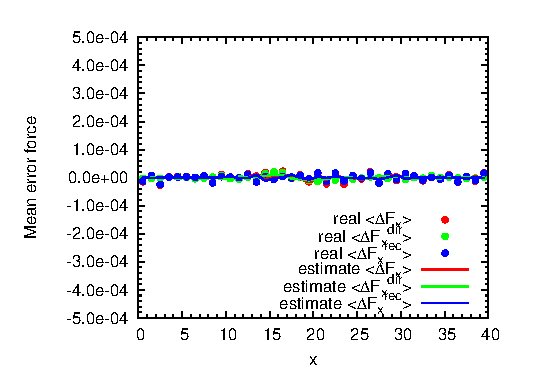
\includegraphics[width=.48\textwidth]{fig/error.one_peak.box40x20x20.b1.000.r3.00.n6.K101x051x051/fig.ana.meanf.eps}
%   \caption{Resulting mean error force}
%   \label{fig:tmp1}
% \end{figure}

% \begin{figure}
%   \centering
%   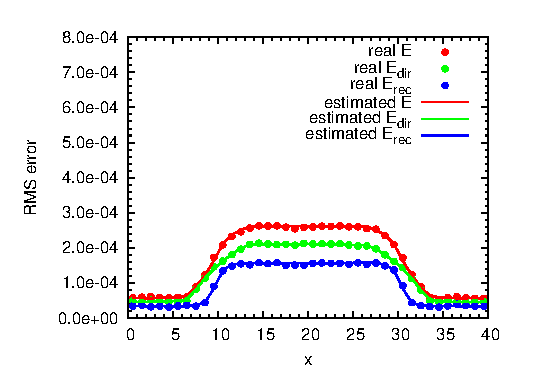
\includegraphics[width=.48\textwidth]{fig/error.one_peak.box40x20x20.b1.000.r3.00.n6.K101x051x051/fig.ik.error.eps}
%   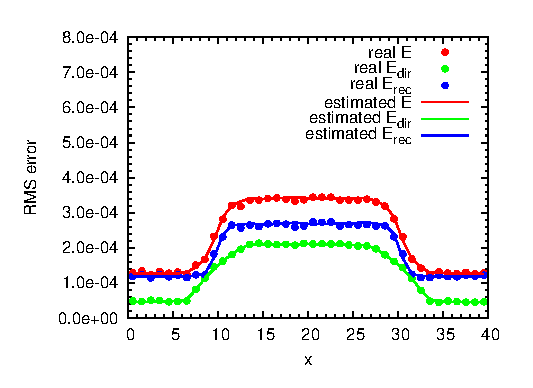
\includegraphics[width=.48\textwidth]{fig/error.one_peak.box40x20x20.b1.000.r3.00.n6.K101x051x051/fig.ana.error.eps}
%   \caption{Resulting RMS errors}
%   \label{fig:tmp2}
% \end{figure}

\subsection{Example 2: seperated positive and negative charge}

\begin{figure}
  \centering
  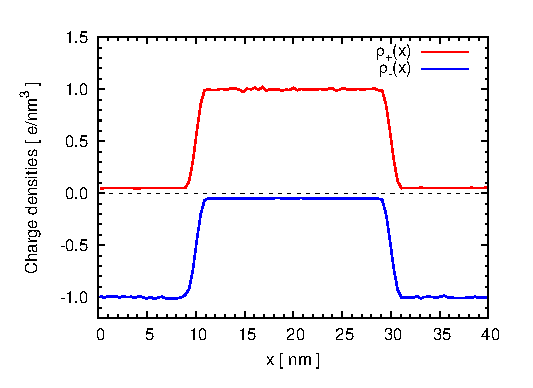
\includegraphics[width=.48\textwidth]{fig/error.two_peaks_sep.box40x20x20.b1.000.r3.00.n6.K101x051x051/fig.rho.eps}
  \caption{Charge distribution of Example 2. The red line
    denotes the positive charge distribution, while the blue line
    denotes the negative charge distribution. Since all distributions
    are uniform on $y$ and $z$ direction, they are plotted as a
    function of $x$.}
  \label{fig:tmp-rho2}
\end{figure}

In this example, 16800 charges are put into a $40\textsf{nm}\times
20\textsf{nm}\times 20\textsf{nm}$ periodic simulation box. Half of
them are carrying a unit positive charge of $+e$, and the other half
are carrying negative charge of $-e$. The position of these charges
are randomly generated subject to density distribution shown in
Fig.~\ref{fig:tmp-rho2}. The nagative charges are seperated from their
counter ions, but the whole system is kept neutral. This case rarely
happen in real simulation, but is serves as a good test of the error
estimates in extreme situations.

\begin{figure}
  \centering
  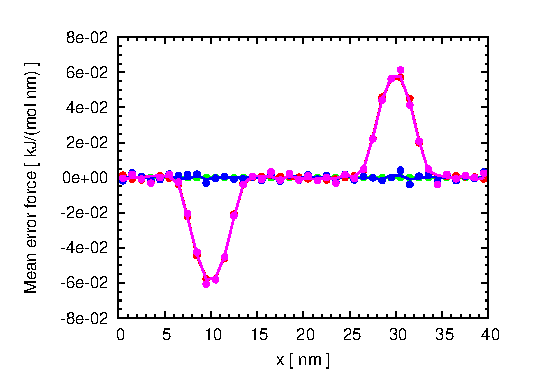
\includegraphics[]{fig/error.two_peaks_sep.box40x20x20.b1.000.r3.00.n6.K101x051x051/fig.ana.ewald.meanf.eps}
  \caption{Example 2: the actual (denoted by dots) and estimated
    (denoted by straight lines) mean error force of the direct part
    $\langle\Delta \v F_{\textrm{dir}}\rangle$ (red), reciprocal part
    of Ewald summation $\langle\Delta \v F_{\textrm{rec}}\rangle$
    (green) and the reciprocal part of the analytical differentiation
    $\langle\Delta \v F^{\textrm{ana}}_{\textrm{rec}}\rangle$
    (blue). The total mean error force of analytical differentiation
    $\langle\Delta \v F^{\textrm{ana}}\rangle$ is given in pink.
    Since the charge distribution is uniform on the $y$ and $z$
    direction, the $y$ and $z$ dimension of the mean error force is
    averaged, and the errors are plotted on $x$ direction. The
    algorithmic parameters are the same as Fig.~\ref{fig:meanf1}.}
  \label{fig:meanf2}
\end{figure}

Fig.~\ref{fig:meanf2} shows the mean error forces of Example 2. All
notations in the Figure are the same as Example 1.  Although the
charge distribution is not usual in this case, the error estimates are
accurate. The two peaks of direct mean force error presented at the
positive-negative interface result from the seperation of the positive
and nagative charges, i.e., a non-vanishing first order charge
distribution $\rho_q$.  Similar phenomena were observed by
Ref.~\cite{wang2012}. The reciprocal mean force error is much smaller
than the direct one, so the contribution to the total mean force error
is not important.

\begin{figure}
  \centering
  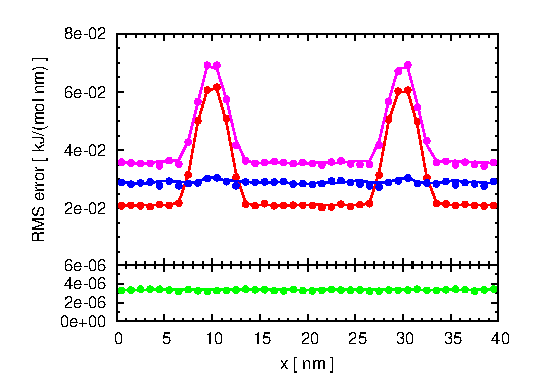
\includegraphics[]{fig/error.two_peaks_sep.box40x20x20.b1.000.r3.00.n6.K101x051x051/fig.ana.ewald.error.eps}
  \caption{Example 2: the actual (denoted by dots) and estimated
    (denoted by straight lines) RMS force error of the direct part
    $\sqrt{\langle\vert\Delta \v F_{\textrm{dir}}(\v
      r)\vert^2\rangle}$ (red), reciprocal part of Ewald summation
    $\sqrt{\langle\vert\Delta \v F_{\textrm{rec}}(\v
      r)\vert^2\rangle}$ (green) and the reciprocal part of the
    analytical differentiation $\sqrt{\langle\vert\Delta \v
      F^{\textrm{ana}}_{\textrm{rec}}\vert^2\rangle}$ (blue). The RMS
    force error of analytical differentiation
    $\sqrt{\langle\vert\Delta \v F^{\textrm{ana}}(\v
      r)\vert^2\rangle}$ is given in pink.  Since the charge
    distribution is uniform on the $y$ and $z$ direction, the $y$ and
    $z$ dimension of the mean error force is averaged, and the errors
    are plotted on $x$ direction. The algorithmic parameters are the
    same as Fig.~\ref{fig:meanf1}.}
  \label{fig:error2}
\end{figure}


Fig. \ref{fig:error2} shows the RMS errors of Example 2. The
corresponding error estimates are accurate. In this case the second
order charge distrubution is a constant, therefore the contribution to
the error is also a constant. The same as Example 1, the reciprocal
error of Ewald sum is much smaller than the direct error and the
reciprocal error of analytical differentiation.  The error peak at the
positive-negative interface, is only 3 times larger than the error of
the bulk regions. For the dispersion interaction, the interfacial
error could be more than one order of maganitude larger than the bulk
error. That is because the direct interaction converges much faster
than the dispersion interaciton ($e^{-r^2}$ v.s. $r^{-6}$).

% \begin{figure}
%   \centering
%   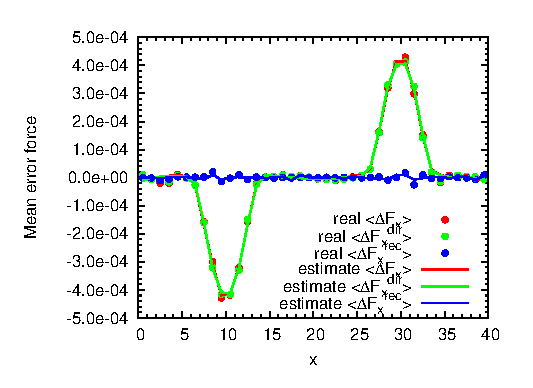
\includegraphics[width=.48\textwidth]{fig/error.two_peaks_sep.box40x20x20.b1.000.r3.00.n6.K101x051x051/fig.ik.meanf.eps}
%   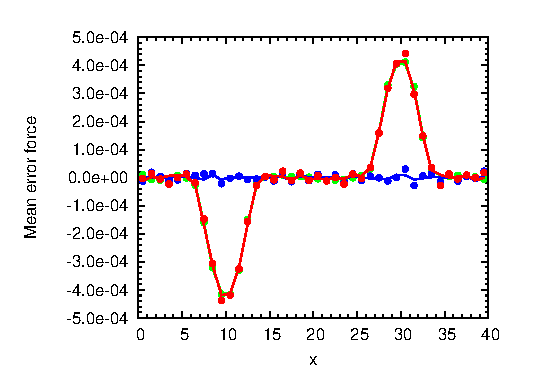
\includegraphics[width=.48\textwidth]{fig/error.two_peaks_sep.box40x20x20.b1.000.r3.00.n6.K101x051x051/fig.ana.meanf.eps}
%   \caption{Resulting mean error force}
%   \label{fig:tmp3}
% \end{figure}

% \begin{figure}
%   \centering
%   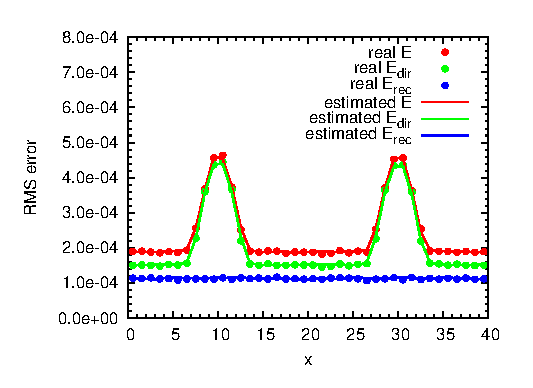
\includegraphics[width=.48\textwidth]{fig/error.two_peaks_sep.box40x20x20.b1.000.r3.00.n6.K101x051x051/fig.ik.error.eps}
%   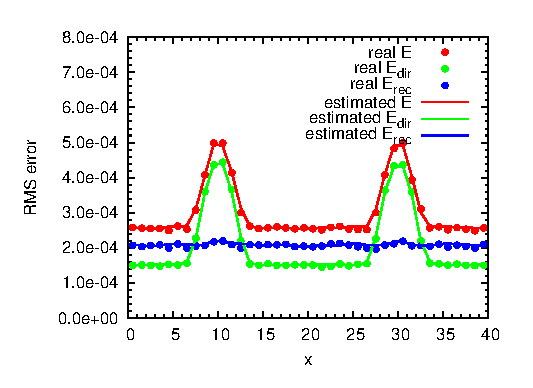
\includegraphics[width=.48\textwidth]{fig/error.two_peaks_sep.box40x20x20.b1.000.r3.00.n6.K101x051x051/fig.ana.error.eps}
%   \caption{Resulting RMS errors}
%   \label{fig:tmp4}
% \end{figure}





\newpage
\appendix
\section{Error estimate of the Ewald summation}




\newpage

\bibliography{ref}{}
\bibliographystyle{unsrt}


\end{document}
